%!TEX root = ../../Main.tex
\graphicspath{{Chapters/Indledning/}}
%-------------------------------------------------------------------------------

\chapter{Indledning}

Nerf guns - legetøjet, der skyder med små skumpile, kommer i alle former og størrelser fra håndholdte pistoler til fuldautomatiske geværer. Der er dog, så vidt gruppen har undersøgt, endnu ikke markedsført en nerf-udgave af en sentry gun. Produktet Big Friendly Gun (BFG) er derfor en automatiseret nerf sentry gun, som automatisk kan sigte efter en brugerbestemt farve, ved hjælp af et intern kamara. Af sikkerhedsmæssige årsager affyrer den ikke skud autonomt, hvorimod brugeren via fjernstyring fra en tilhørende PC-app skal bede om at affyre skud. Udover automatisk at sigte efter farver, vil det også være muligt manuelt at fjernstyre kanonen via PC-appen.

Nedenfor, på figur \ref{fig:rigt_billede} ses et overblik over systemets funktionalitet, med et konceptbillede.

\begin{figure}[H]
	\centering
	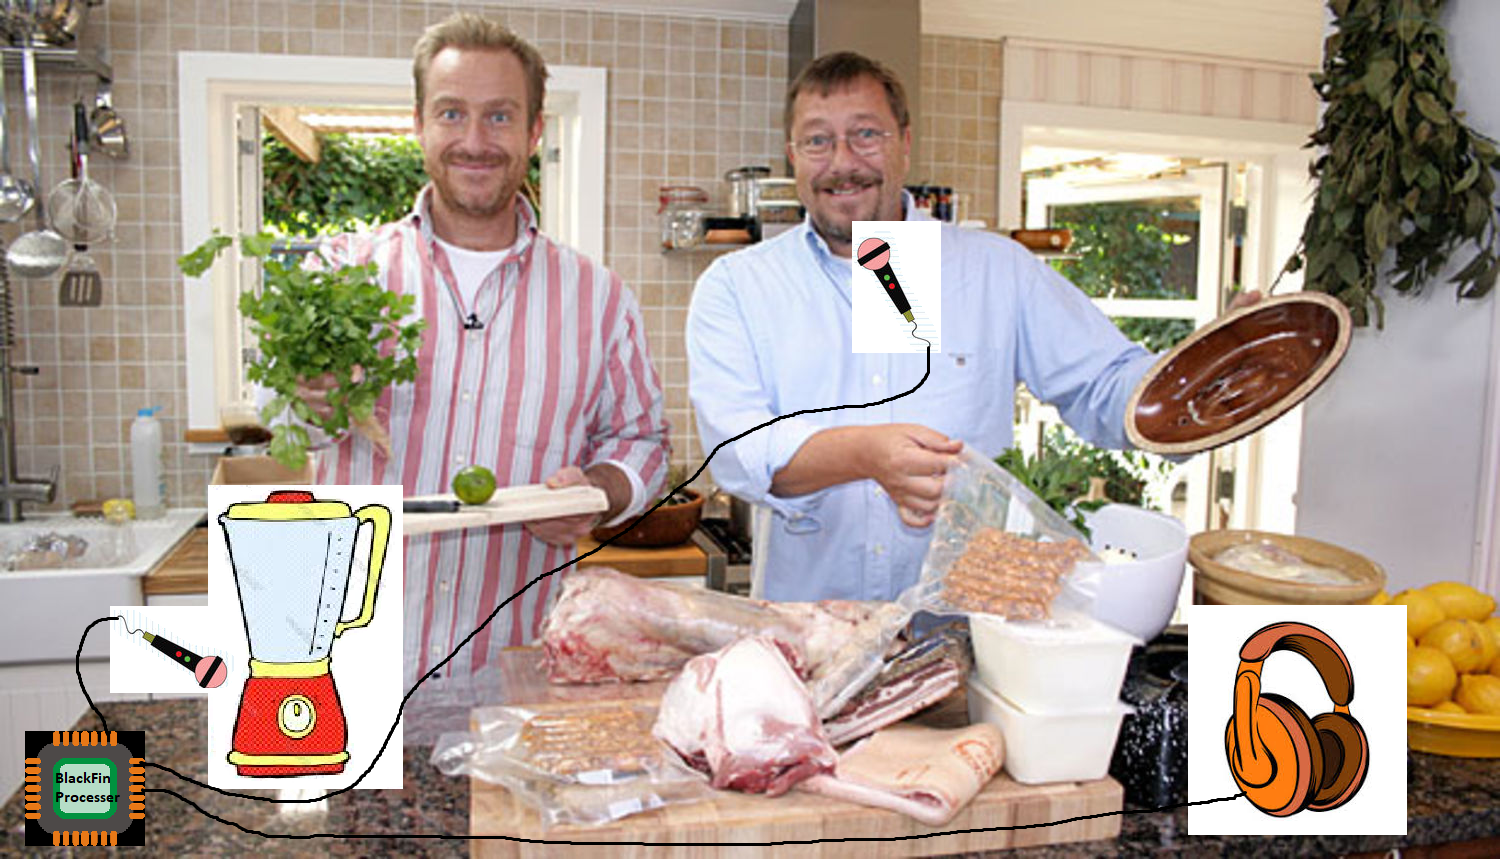
\includegraphics[width = 400pt]{Img/Konceptbillede}
	\caption{Konceptbillede for BFG}
	\label{fig:rigt_billede}
\end{figure}

Med udgangspunkt i brugerens behov vil der blive opstillet en række brugsscenarier, der beskriver brugerens interaktion med systemet. Disse scenarier vil sammen med en række veldefinerede krav og afgrænsninger, danne grundlaget for designet af alle dele af systemet. I selve designfasen vil systemet blive opdelt i mindre dele, kaldet moduler, for at lette overskueligheden og gøre systemet mere fleksibelt og skalerbart.  \\ 

\newpage






\section{Læsevejledning}

Denne sektion har til formål at give et kort overblik over hvad rapporten indeholder, og hvor man kan læse om de forskellige dele:

\textbf{Kapitel 1-7} vil give en overordnet præsentation af produktet for dette semesterprojekt. Yderligere vil man kunne læse om funktionaliteten og formålet med produktet, samt hvad produktet overordnet består af. 

\textbf{Kapitel 8} vil give et overblik over de forskellige moduler og deres overordnede funktionalitet, som til sammen danner BFG og dermed hele systemet.

\textbf{Kapitel 9} danner overblik over de forskellige kommunikationsprotokoller der bliver brugt i BFG. Yderligere bliver der begrundet for de valgte kommunikatonsprotokoller.

\textbf{Kapitel 10} beskriver PC-App modulets funktionalitet og overvejelser om dette. Dette inkluderer også overvejelser om design og beskrivelse af implementeringen for PC-Appen og alt der hører under dets modul.

\textbf{Kapitel 11} beskriver drejemodulet og dets funktionalitet. Yderligere forklarer afsnittet om overvejelser angående modulet samt design og implementeringsfasen. 

\textbf{Kapitel 12} danner overblik over kontrolmodulet og dets funktionalitet. Desuden beskriver kapitlet kommunikationsprotokollerne og billedeprocesseringen som er implementeret.

\textbf{Kapitel 13} giver indsigt i affyringsmodulet og overvejelse om forskellige ting som indgår i modulet. 

\textbf{Kapitel 14} giver et kort indblik i overvejelser om EMC i BFG.

\textbf{Kapitel 15} beskriver systemets integrationstest.

\textbf{Kapitel 16-17} fungerer som en afrunding på denne rapport. Her bliver der præsenteret et resultat, samt en diskussion om denne, hvorefter der følger en endelig konklusion på semesterprojektet og dets rapport.

